\documentclass[prl, twocolumn, ,superscriptaddress]{revtex4-1}

\usepackage{graphicx}
\usepackage{xcolor}

\newcommand{\letter}{Manuscript}

\begin{document}
\title{Surface code quantum computing in a network with timing errors}

\author{Joe O'Gorman}
\affiliation{Department of Materials, Oxford University}
\author{Naomi H. Nickerson}
\email{n.nickerson11@imperial.ac.uk}
\affiliation{Quantum Optics and Laser Science, Blackett Laboratory, Imperial College London, Prince Consort Road, London SW7 2AZ, United Kingdom}


\begin{abstract}
A networked approach to quantum computing made up of small cells of well controlled qubits, 
connected together by long range photonics connections has been shown to be a reasonable 
approach to achieinvg scalability with matter based qubit systems, such as trapped ions.  
This approach overcomes many of the challenges faced by matter based qubit systems allowing
 complex architectures, long range connections, and ... without any increased complexity in the
  cell design. Performing operations across the network - such as the four-body measurements
   required to implement the surface code - require the ability to keep time between remote cells. 
   Here we identify the nature of errors that arise from inaccurate time keeping, and find thresholds
    for what level of inaccuracy can be tolerated by error correction with the surface code. 
\end{abstract}

\maketitle


Error correcting codes, such as the surface code, are based on the repeated projective measurement 
of the stabilizers of the code. In order to understand how timing errors will affect the implementation the code, 
we must identify how these parity measurements will be affected. We consider the case where we aim to 
measure the Pauli $Z$ operator on a single qubit, but instead measure in some slightly rotated basis 
$\cos\theta Z+\sin\theta X$. The projection into this rotated basis, can be viewed as a rotation
of the state, followed by the ideal Z projection, and a finally a rotation back into the original basis. 
Thus we can write this rotated projection as,

\[
P\left(\theta\right)=R^{\dagger}\left(\theta\right)\hat{P}_{Z}R\left(\theta\right)\]


Where $P_{Z}$ and $P\mbox{\ensuremath{\left(\theta\right)}}$ are
taken to be even projection operators into the bases $Z$ and $\cos\theta Z+\sin\theta X$ respectively, and 
the rotation operator $R\left(\theta\right)=R_{y}\left(\theta\right)=\cos\frac{\theta}{2}\mathbb{I}-i\sin\frac{\theta}{2}Y$.
Defining $C=\cos\frac{\theta}{2}$ and $S=\sin\frac{\theta}{2}$, we can write this explicitly as,

\[
P\left(\theta\right)  =  C^{2}P_{Z}+S^{2}YP_{Z}Y+iSC\left[YP_{Z}-P_{Z}Y\right]
\]


Using the relationship $P_{Z}Y=YP_{Z,odd}$ we can write,

\begin{equation}
\label{eq:p_theta}
P\left(\theta\right)  =  C^{2}P_{Z}+S^{2}P_{Z,odd}+iSCY\left[P_{Z}-P_{Z,odd}\right]
\end{equation}

%\begin{eqnarray*}
%P\left(\theta\right) & = & C^{2}P_{Z}+S^{2}P_{Z,odd}+iSCY\left[P_{Z}-P_{Z,odd}\right]\\
%P\left(\theta\right) & = & C^{2}P_{Z}+S^{2}P_{Z,odd}+iSC\left[P_{Z,odd}-P_{Z}\right]Y\end{eqnarray*}

This operator exactly describes the effect of projecting into the rotated basis. However to understand the effect of 
errors, we must also include our uncertainty in the value of $\theta$, which is drawn from some probability distribution that
describes our noise model. If an observed even measurement outcome corresponds to the projector $P\left(\theta\right)$ being 
applied to the state with probability $q\left(\theta\right)$ then we obtain the density matrix describing the output state after 
this noisy measurement by integrating over this distribution.

\begin{eqnarray*}
\rho_{measured} & = & \int_{\theta} q\left(\theta\right)P\left(\theta\right)\rho P\left(\theta\right)d\theta\\
\end{eqnarray*}

Using equation~\ref{eq:p_theta}, we can then write:

\[
\rho_{measured}  = \int_{\theta} q(\theta) \left[ C^{4} \rho_1 + iC^{3}S \rho_2 +C^{2}S^{2} \rho_3 +iCS^{3} \rho_4 + S^{4} \rho_5 \right] d\theta
\]
 
Where the five terms are given by,
 
 \begin{eqnarray*}
 \rho_1 & = & \rho_{even}\\
 \rho_2 & = & -\rho_{even}Y+Y\rho_{even}-YP_{Z,odd}\rho P_{Z}+P_{Z}\rho P_{Z,odd}Y\\
 \rho_3 & = & Y\rho_{odd}Y+Y\rho_{even}Y+P_{Z}\rho P_{Z,odd}+P_{Z,odd}\rho P_{Z}-YP_{Z}\rho P_{Z,odd}Y-YP_{Z,odd}\rho P_{Z}Y\\
 \rho_4 & = & -Y\rho_{odd}+\rho_{odd}Y-P_{Z,odd}\rho P_{Z}Y+YP_{Z}\rho P_{Z,odd}\\
 \rho_5 & = & \rho_{odd}
 \end{eqnarray*}

and we have used the definitions: $\rho_{even}=P_{Z}\rho P_{Z}$, and $\rho_{odd}=P_{Z,odd}\rho P_{Z,odd}$.

%\begin{eqnarray*}
%\rho_{measured} & = & \int q\left(\theta\right)P\left(\theta\right)\rho P\left(\theta\right)d\theta\\
% &  & C^{4}\rho_{even}+S^{4}\rho_{odd}\\
% &  & +iC^{3}S\left[-\rho_{even}Y+Y\rho_{even}-YP_{Z,odd}\rho P_{Z}+P_{Z}\rho P_{Z,odd}Y\right]\\
% &  & +C^{2}S^{2}\left[Y\rho_{odd}Y+Y\rho_{even}Y+P_{Z}\rho P_{Z,odd}+P_{Z,odd}\rho P_{Z}-YP_{Z}\rho P_{Z,odd}Y-YP_{Z,odd}\rho P_{Z}Y\right]\\
% &  & +iCS^{3}\left[-Y\rho_{odd}+\rho_{odd}Y-P_{Z,odd}\rho P_{Z}Y+YP_{Z}\rho P_{Z,odd}\right]\end{eqnarray*}
%

% \begin{eqnarray*}
% A & = & C^{4}P_{Z}\rho P_{Z}+S^{4}\hat{P_{Z,odd}}\rho\hat{P_{Z,odd}}\\
% B & = & iC^{3}S\left[P_{Z}\rho P_{Z,odd}Y-P_{Z}\rho P_{Z}Y+YP_{Z}\rho P_{Z}-YP_{Z,odd}\rho P_{Z}\right]\\
% C & = & C^{2}S^{2}[P_{Z}\rho P_{Z,odd}+P_{Z,odd}\rho P_{Z}-YP_{Z}\rho P_{Z,odd}YY\\
% &  & \ \ \ \ \ \ \ \ \ \  \  +YP_{Z,odd}\rho P_{Z,odd}+YP_{Z}\rho P_{Z}Y -YP_{Z,odd}\rho P_{Z}Y]\\
% D & = & iCS^{3}\left[P_{Z,odd}\rho P_{Z,odd}Y-P_{Z,odd}\rho P_{Z}Y+YP_{Z}\rho P_{Z,odd}-YP_{Z,odd}\rho P_{Z,odd}\right]
% \end{eqnarray*}
% 
 
%\begin{eqnarray*}
%\rho_{measured} & = & \int q\left(\theta\right)R^{\dagger}\left(\theta\right)P_{Z}R\left(\theta\right)\rho R^{\dagger}\left(\theta\right)P_{Z}R\left(\theta\right)d%%\theta\end{eqnarray*}

To understand how these erroneous terms manifest themselves in our final density matrix after projection, we must consider the nature of our distribution of errors, $q(\theta)$. We first find the form of the errors in the case that $q(\theta)$ is symmetric, and has no systematic component. Later, we will show how this result can be straightforwardly extended to the case of systematic errors. 

When $q(\theta)$ is symmetric about $\theta=0$ the asymmetric terms in the integral, $\rho_2$ and $\rho_4$, vanish, and we are left
with,

%\begin{eqnarray*}
%\rho_{measured} & = & \int q\left(\theta\right)\{C^{4}\rho_{even}+S^{4}\rho_{odd}+C^{2}S^{2}\left[Y\rho_{odd}Y+Y\rho_{even}Y\right]\\
% &  & +C^{2}S^{2}\left[P_{Z}\rho P_{Z,odd}+P_{Z,odd}\rho P_{Z}-YP_{Z}\rho P_{Z,odd}Y-YP_{Z,odd}\rho P_{Z}Y\right]\}d\theta\end{eqnarray*}

\[
\rho_{measured}  = \int_{\theta} q(\theta) \left[ C^{4} \rho_1 +C^{2}S^{2} \rho_3 + S^{4} \rho_5 \right] d\theta
\]
 
The remaining terms in the integral, can all be easily understood physically, with the exception of $\rho_3$, which contains terms such as $P_{Z,odd}\rho P_{Z}$. By applying a Z gate to the qubit with 50\% probability, we split the density matrix into a sum of two parts, where these terms have opposite signs in each part. Overall then these problematic terms now cancel, leaving us with a form which can be more straightforwardly simulated. 
% What actually does this correspond to physically? Can we say that it would actually be bad to leave these here, and not just that they are difficult to simulate?

Under these conditions, the noisy measurement can then be written as a superoperator,

\[
\mathcal{S}\left(\rho\right)=\sum p_{i}K_{i}\rho K_{i}^{\dagger}
\]

Where the Kraus operators, $K_i$, are given by the remaining terms of $\rho_1$, $\rho_3$ and $\rho_5$, and the probabilities, $p_i$, are found by integrating the constants over $q(\theta)$. These are summarized in table~\ref{table:superoperator}.

%\[
%\rho_{measured} = A \rho_{odd} + B \rho_{even} + C \left[ Y\rho_{odd}Y+Y\rho_{even}Y\right]
%\]
%
%Where,
%
% \begin{eqnarray*}
% A & = & \int q\left(\theta\right)C^{4}d\theta \\
% B & = & \int q\left(\theta\right)S^{4}d\theta \\
% C & = & \int q\left(\theta\right)C^{2}S^{2}d\theta \\
% \end{eqnarray*}
%
%
%
%
%So we can write the resultant channel as a superoperator 
%


\begin{figure}
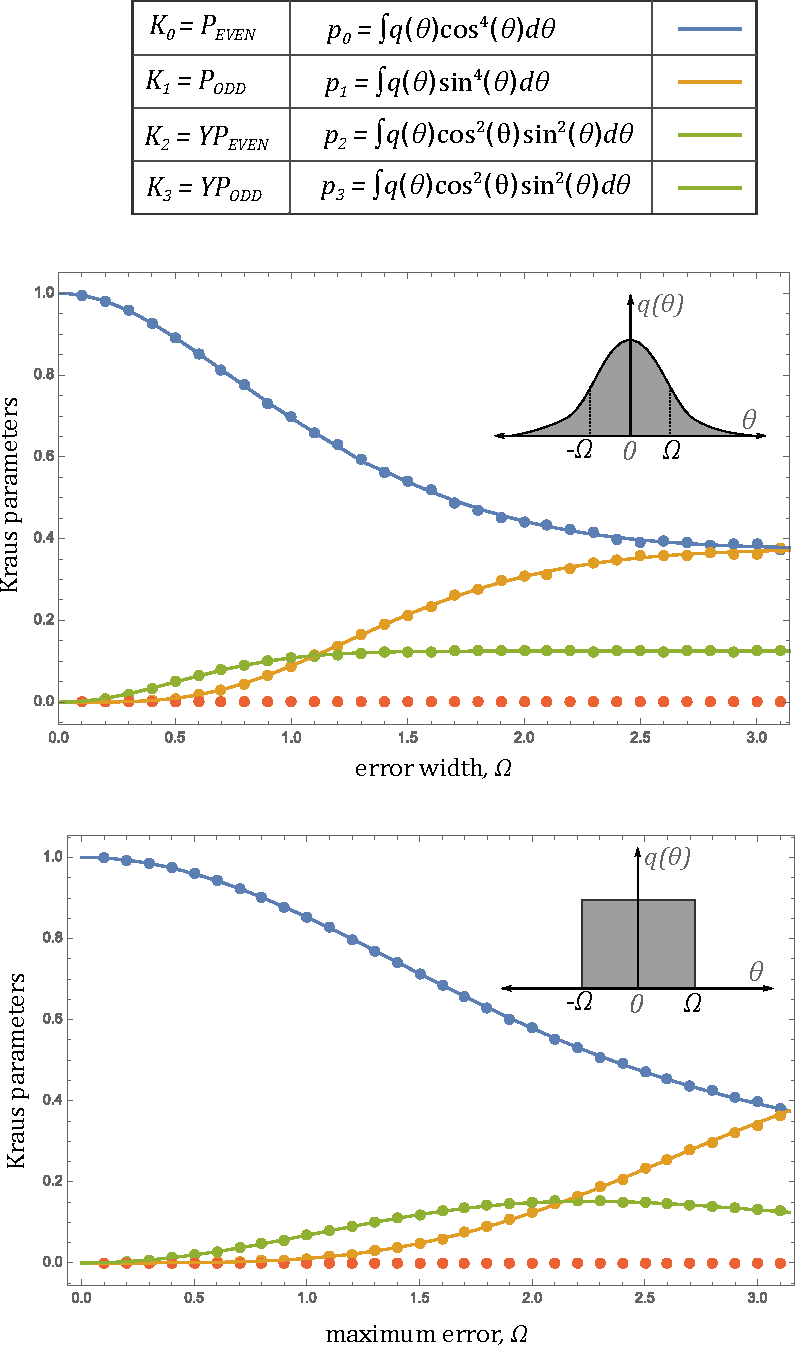
\includegraphics[width=0.4\textwidth]{single_qubit_plots_1.pdf}
\caption{Magnitude of the terms of the super operator under a) Normally distributed noise b) uniformly distributed noise. The solid lines show the value calculated directly from the integrals in the summary table. Data points show the results of simulation over $10^4$ trials, where the value of $\theta$ was sampled from the distribution $q(\theta)$ in each trial. Red data points show the remaining amplitude of the simulated density matrix, not described by any of the four Kraus operators. This is vanishingly small, reinforcing that the model is a full description of the resulting errors.}
\label{table:superoperator}
\end{figure}

%
%
%\label{table:superoperator}
%\begin{tabular}{|c|c|}
%\hline 
% & \tabularnewline
%\hline
%\hline 
%$p_{0}=\mbox{\ensuremath{\left[\int q\left(\theta\right)C^{4}d\theta\right]}}$ & $K_{0}=P_{Z}$\tabularnewline
%\hline 
%$p_{1}=\left[\int q\left(\theta\right)S^{4}d\theta\right]$ & $K_{1}=P_{Z,odd}$\tabularnewline
%\hline 
%$p_{2}=\left[\int q\left(\theta\right)C^{2}S^{2}d\theta\right]$ & $K_{2}=YP_{Z,odd}$\tabularnewline
%\hline 
%$p_{3}=\left[\int q\left(\theta\right)C^{2}S^{2}d\theta\right]$ & $K_{3}=YP_{Z}$\tabularnewline
%\hline
%\end{tabular}


\subsection{Case of systematic errors }

If systematic error is present then the probability function, $q_{sys}\left(\theta\right)$,
describing the distribution of the error does not average to zero,
but rather $\int q_{sys}\left(\theta\right)d\theta=\bar{\theta}$.
By changing variables to $\phi=\theta-\bar{\theta}$

\begin{eqnarray*}
\rho_{measured} & = & \int_{\theta}q_{sys}\left(\theta\right)P\left(\theta\right)\rho P\left(\theta\right)d\theta\\
 & = & \int_{\phi}q_{sys}\left(\phi+\bar{\theta}\right)P\left(\phi+\bar{\theta}\right)\rho P\left(\phi+\bar{\theta}\right)d\phi\\
 & = & \int_{\phi}q_{rand}\left(\phi\right)R^{\dagger}\left(\phi+\bar{\theta}\right)\hat{P}_{Z}R\left(\phi+\bar{\theta}\right)\rho R^{\dagger}\left(\phi+\bar{\theta}\right)\hat{P}_{Z}R\left(\phi+\bar{\theta}\right)d\phi\\
 & = & R\left(\bar{\theta}\right)\left\{ \int_{\phi}q_{rand}\left(\phi\right)R^{\dagger}\left(\phi\right)\hat{P}_{Z}R\mbox{(\ensuremath{\phi})}\rho_{\bar{\theta}}R^{\dagger}\left(\phi\right)\hat{P}_{Z}R\left(\phi\right)d\phi\right\} R^{\dagger}\left(\bar{\theta}\right)\\
 & = & R\left(\bar{\theta}\right)\left\{ \int_{\phi}q_{rand}\left(\phi\right)P\left(\phi\right)\rho_{\bar{\theta}}P\left(\phi\right)d\phi\right\} R^{\dagger}\left(\bar{\theta}\right)\end{eqnarray*}


where $\rho_{\bar{\theta}}=R\mbox{(\ensuremath{\bar{\theta)}\rho}}R^{\dagger}\mbox{(\ensuremath{\bar{\theta)}}}$

So with systematic errors, we can also write the effect as a superoperators
where a fixed rotation is followed by an application of random errors
which average to zero. 



\bibstyle{plain}
\begin{thebibliography}{60}


\end{thebibliography}




\end{document}















